\chapter{explosions} 
\label{sec:presets}
\lstset{style=6502Style}
Text here
\begin{definition}[Jeffrey Says]
\setlength{\intextsep}{0pt}%
\setlength{\columnsep}{3pt}%
\begin{wrapfigure}{l}{0.12\textwidth}

\includegraphics[width=\linewidth]{src/callout/psych.png} 
\end{wrapfigure}
\small
The "E" key toggles between "explosion" and "normal" drawing mode.

In "explosion" mode the cursor leaves a trail of "explosions" rather than the
usual image of the lightform-primitive.  This mode is usually most effective if
you are using a pulsed stream (see PULSE RATE later).
\end{definition}
\clearpage

\clearpage
\begin{minipage}[b]{0.48\linewidth}
\begin{figure}[H]                                                          
  \centering                                                             
  \begin{adjustbox}{width=5cm,center}                                   
  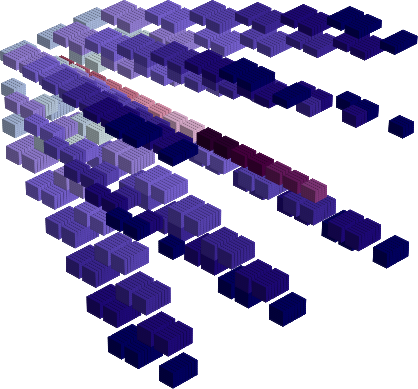
\includegraphics[width=5cm]{src/colorspace_presets/preset18-45.png}%           
  \end{adjustbox}                                                        
\caption*{Preset 18.}                                           
\end{figure}                                                               
\end{minipage}
\hspace{0.1cm}
\begin{minipage}[b]{0.48\linewidth}                            
\begin{lstlisting}[basicstyle=\ttfamily\tiny]
preset18
  .BYTE $02 ; cursorSpeed
  .BYTE $01 ; vectorMode
  .BYTE $01 ; speedBoostAdjust
  .BYTE $0D ; currentPatternIndex
  .BYTE $05 ; verticalResolutionSPAC
  .BYTE $01 ; pulseSpeed
  .BYTE $02 ; currentPulseWidth
  .BYTE $10 ; smoothingDelay
  .BYTE $01 ; currentSymmetry
  .BYTE $02 ; screenMode
  .BYTE $40 ; bufferLength
  .BYTE $00 ; stroboscopicsEnabled
  .BYTE $02 ; stroboFlashRate
  .BYTE BLACK0,ULTRAMARINE_BLUE0 ; colorPalette
  .BYTE ULTRAMARINE_BLUE2,ULTRAMARINE_BLUE4 ; colorPalette
  .BYTE ULTRAMARINE_BLUE6,ULTRAMARINE_BLUE8 ; colorPalette
  .BYTE ULTRAMARINE_BLUE10,MEDIUM_BLUE0 ; colorPalette
  .BYTE $00,$00,$00,$00,$00,$00,$00,$02 ; oozeRates
  .BYTE $01,$01,$01,$01,$01,$01,$01,$01 ; oozeSteps
  .BYTE $0F,$0F,$0F,$0F,$0F,$0F,$0F,$0F ; oozeCycles
  .BYTE $00 ; explosionMode
\end{lstlisting}
\end{minipage}

\vspace*{1.5cm}

\begin{minipage}[b]{0.48\linewidth}
\begin{figure}[H]                                                          
  \centering                                                             
  \begin{adjustbox}{width=5cm,center}                                   
  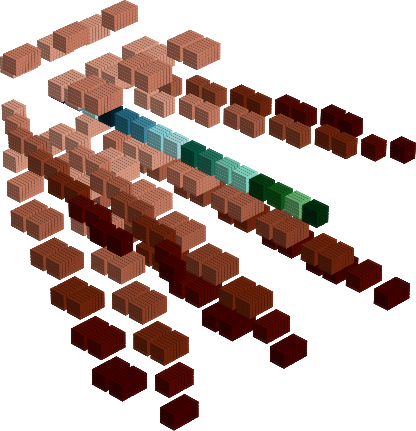
\includegraphics[width=5cm]{src/colorspace_presets/preset26-45.png}%           
  \end{adjustbox}                                                        
\caption*{Preset 26.}                                           
\end{figure}                                                               
\end{minipage}
\hspace{0.1cm}
\begin{minipage}[b]{0.48\linewidth}                                                                         
\begin{lstlisting}[basicstyle=\ttfamily\tiny]
preset26
  .BYTE $01 ; cursorSpeed
  .BYTE $01 ; vectorMode
  .BYTE $01 ; speedBoostAdjust
  .BYTE $0E ; currentPatternIndex
  .BYTE $05 ; verticalResolutionSPAC
  .BYTE $06 ; pulseSpeed
  .BYTE $00 ; currentPulseWidth
  .BYTE $7B ; smoothingDelay
  .BYTE $01 ; currentSymmetry
  .BYTE $00 ; screenMode
  .BYTE $24 ; bufferLength
  .BYTE $02 ; stroboscopicsEnabled
  .BYTE $02 ; stroboFlashRate
  .BYTE BLACK9,DARK_ORANGE1 ; colorPalette
  .BYTE DARK_ORANGE2,DARK_ORANGE4 ; colorPalette
  .BYTE DARK_ORANGE6,DARK_ORANGE8 ; colorPalette
  .BYTE DARK_ORANGE10,DARK_ORANGE12 ; colorPalette
  .BYTE $00,$00,$00,$00,$00,$00,$00,$00 ; oozeRates
  .BYTE $01,$01,$01,$01,$01,$01,$01,$01 ; oozeSteps
  .BYTE $0F,$0F,$0F,$0F,$0F,$0F,$0F,$0F ; oozeCycles
  .BYTE $00 ; explosionMode
\end{lstlisting}
\end{minipage}
\clearpage

\begin{minipage}[b]{0.48\linewidth}
\begin{figure}[H]                                                          
  \centering                                                             
  \begin{adjustbox}{width=5cm,center}                                   
  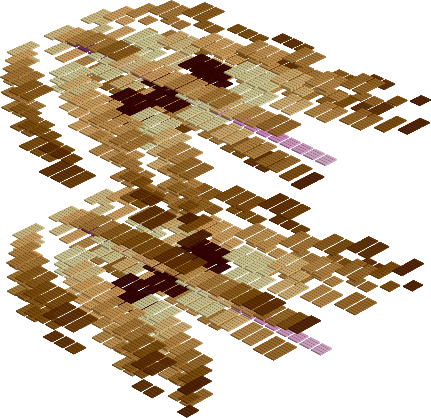
\includegraphics[width=5cm]{src/colorspace_presets/preset46-45.png}%           
  \end{adjustbox}                                                        
\caption*{Preset 46.}                                           
\end{figure}                                                               
\end{minipage}
\hspace{0.1cm}
\begin{minipage}[b]{0.48\linewidth}                                       
\begin{lstlisting}[basicstyle=\ttfamily\tiny]
preset46
  .BYTE $01 ; cursorSpeed
  .BYTE $01 ; vectorMode
  .BYTE $02 ; speedBoostAdjust
  .BYTE $14 ; currentPatternIndex
  .BYTE $05 ; verticalResolutionSPAC
  .BYTE $04 ; pulseSpeed
  .BYTE $01 ; currentPulseWidth
  .BYTE $04 ; smoothingDelay
  .BYTE $01 ; currentSymmetry
  .BYTE $06 ; screenMode
  .BYTE $40 ; bufferLength
  .BYTE $00 ; stroboscopicsEnabled
  .BYTE $02 ; stroboFlashRate
  .BYTE BLACK0,RUST6 ; colorPalette
  .BYTE RUST8,RUST10 ; colorPalette
  .BYTE RUST12,RUST14 ; colorPalette
  .BYTE RED_ORANGE0,RED_ORANGE2 ; colorPalette
  .BYTE $00,$02,$02,$02,$02,$02,$02,$02 ; oozeRates
  .BYTE $01,$01,$01,$01,$01,$01,$01,$01 ; oozeSteps
  .BYTE $0F,$0F,$0F,$0F,$0F,$0F,$0F,$0F ; oozeCycles
  .BYTE $00 ; explosionMode
\end{lstlisting}
\end{minipage}

\vspace*{1.5cm}

\begin{minipage}[b]{0.48\linewidth}
\begin{figure}[H]                                                          
  \centering                                                             
  \begin{adjustbox}{width=5cm,center}                                   
  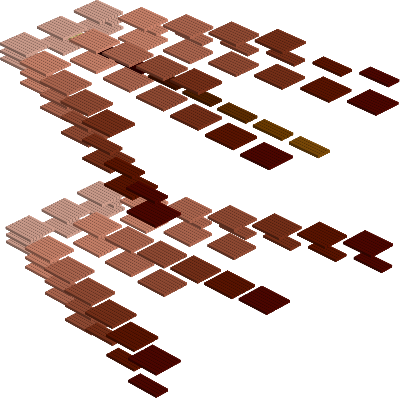
\includegraphics[width=5cm]{src/colorspace_presets/preset76-45.png}%           
  \end{adjustbox}                                                        
\caption*{Preset 76.}                                           
\end{figure}                                                               
\end{minipage}
\hspace{0.1cm}
\begin{minipage}[b]{0.48\linewidth}                                       
\begin{lstlisting}[basicstyle=\ttfamily\tiny]
preset76
  .BYTE $01 ; cursorSpeed
  .BYTE $01 ; vectorMode
  .BYTE $02 ; speedBoostAdjust
  .BYTE $01 ; currentPatternIndex
  .BYTE $02 ; verticalResolutionSPAC
  .BYTE $04 ; pulseSpeed
  .BYTE $00 ; currentPulseWidth
  .BYTE $06 ; smoothingDelay
  .BYTE $04 ; currentSymmetry
  .BYTE $00 ; screenMode
  .BYTE $40 ; bufferLength
  .BYTE $01 ; stroboscopicsEnabled
  .BYTE $01 ; stroboFlashRate
  .BYTE BLACK5,DARK_ORANGE1 ; colorPalette
  .BYTE DARK_ORANGE2,DARK_ORANGE4 ; colorPalette
  .BYTE DARK_ORANGE6,DARK_ORANGE8 ; colorPalette
  .BYTE DARK_ORANGE10,DARK_ORANGE12 ; colorPalette
  .BYTE $00,$14,$14,$14,$14,$14,$14,$14 ; oozeRates
  .BYTE $01,$01,$01,$01,$01,$01,$01,$01 ; oozeSteps
  .BYTE $0F,$00,$00,$00,$00,$00,$00,$00 ; oozeCycles
  .BYTE $00 ; explosionMode
\end{lstlisting}
\end{minipage}
\clearpage

\textbf{Lines 1189-1231. \icode{\textbf{MaybeEKeyPressed}}} 
\begin{lstlisting}
MaybeEKeyPressed   
        CMP #KEY_E
        BNE MaybeCtrlQPressed

        ; E=Explosion mode on/off 
        LDA explosionMode
        EOR #$80
        STA explosionMode
        AND #$80
        BNE UpdateExplosionModeStatus
        LDX #NORMAL_PATTERN_MODE
        JMP UpdateStatusLine

UpdateExplosionModeStatus   
        LDX #EXPLOSION_MODE_ON
        JMP UpdateStatusLine

\end{lstlisting}
\textbf{Lines 1189-1231. \icode{\textbf{explosionModeArray}}} 
\begin{lstlisting}
explosionModeArray   
        .BYTE $43,$48,$33,$31,$0A,$09,$55,$C0
        .BYTE $77,$0D,$4B,$45,$59,$39,$0B,$30
        .BYTE $55,$C0,$97,$0D,$4B,$45,$59,$31
        .BYTE $30,$0A,$0D,$55,$C0,$91,$0E,$53
        .BYTE $59,$4E,$43,$0B,$0F,$55,$C0,$7D
        .BYTE $0F,$5A,$5A,$54,$4F,$50,$08,$3B
        .BYTE $55,$C0,$9F,$0D,$4B,$54,$0B,$65
        .BYTE $55,$C0,$AA,$0D,$4B,$45,$59,$31
\end{lstlisting}

\clearpage

\textbf{Lines 1189-1231. \icode{\textbf{MaybeEKeyPressed}}:} 
text
\clearpage

\textbf{Lines 1189-1231. \icode{\textbf{MainGameLoop}}} 
\begin{lstlisting}
MainGameLoop

        ...
        LDA explosionModeArray,X
        AND #$0F
        CMP #$0F
        BNE SetUpExplosionPaint
        STX FR2
        BEQ GoBackToStartOfLoop

SetUpExplosionPaint   
        LDA explosionModeArray,X
        STA currentPaintState
        AND #$07
        STA pixelsToPaint
        LDA pixelXPositionArray,X
        STA currentPixelXPosition
        LDA pixelYPositionArray,X
        STA currentPixelYPosition
        LDA patternIndexArray,X
        STA patternIndex
        LDA symmetrySettingForStepCount,X
        STA currentSymmetrySetting
        LDA bottomMostYPosArray,X
        STA currentBottomMostYPos
        LDA initialFramesRemainingToNextPaintForStep,X
        STA framesRemainingToNextPaintForStep,X
        DEC explosionModeArray,X
        JSR PaintStructureAtCurrentPosition

GoBackToStartOfLoop
        LDA selectedModePreventsForegroundDrawing
        BEQ MainGameLoop
        LDA #$00
        STA SDMCTL   ;SDMCTL  shadow for DMACTL ($D400)
        JSR GenerateDisplayList
        LDA #$00
        STA selectedModePreventsForegroundDrawing
        JMP MainGameLoop
\end{lstlisting}

\clearpage

\textbf{Lines 1189-1231. \icode{\textbf{MainGameLoop}}:} 
text

\clearpage
\textbf{Lines 1189-1231. \icode{\textbf{PaintExplosionMode}}} 
\begin{lstlisting}
explosionMode   .BYTE $00
;------------------------------------------------------
; PaintExplosionMode
;------------------------------------------------------
PaintExplosionMode
        LDA currentPaintState
        AND #$77
        STA currentPaintState
        LDA #$0A
        SEC 
        SBC pixelsToPaint
        STA paintOffset
        JSR PaintExplosionPixels
        DEC paintOffset
        LDA #$10
        STA currentPaintState
        STA ATRACT   ;ATRACT  screen attract counter
        JSR PaintExplosionPixels
        RTS 

\end{lstlisting}

\clearpage

\textbf{Lines 1189-1231. \icode{\textbf{PaintExplosionMode}}:} 
text
\clearpage



\textbf{Lines 1189-1231. \icode{\textbf{PaintExplosionPixels}}} 
\begin{lstlisting}
PaintExplosionPixels
        LDA currentPixelXPosition
        PHA 
        STA previousPixelXPosition
        LDA currentPixelYPosition
        PHA 
        SEC 
        SBC paintOffset
        STA previousPixelYPosition
        STA currentPixelYPosition
        JSR PaintPixelForCurrentSymmetry
        LDA currentPixelXPosition
        CLC 
        ADC paintOffset
        STA currentPixelXPosition
        STA previousPixelXPosition
        LDA currentPixelYPosition
        STA previousPixelYPosition
        JSR PaintPixelForCurrentSymmetry
        LDA currentPixelXPosition
        STA previousPixelXPosition
        PLA 
        PHA 
        STA previousPixelYPosition
        JSR PaintPixelForCurrentSymmetry
        LDA currentPixelXPosition
        STA previousPixelXPosition
        PLA 
        PHA 
        CLC 
        ADC paintOffset
        STA previousPixelYPosition
        STA currentPixelYPosition
        JSR PaintPixelForCurrentSymmetry

\end{lstlisting}

\clearpage

\textbf{Lines 1189-1231. \icode{\textbf{PaintExplosionPixels}}:} 
text
\clearpage



\textbf{Lines 1189-1231. \icode{\textbf{PaintExplosionPixels}} cont.} 
\begin{lstlisting}
        ; PaintExplosionPixels continued..
        LDA currentPixelXPosition
        SEC 
        SBC paintOffset
        STA currentPixelXPosition
        STA previousPixelXPosition
        LDA currentPixelYPosition
        STA previousPixelYPosition
        JSR PaintPixelForCurrentSymmetry
        LDA currentPixelXPosition
        SEC 
        SBC paintOffset
        STA currentPixelXPosition
        STA previousPixelXPosition
        LDA currentPixelYPosition
        STA previousPixelYPosition
        JSR PaintPixelForCurrentSymmetry
        LDA currentPixelXPosition
        STA previousPixelXPosition
        LDA currentPixelYPosition
        SEC 
        SBC paintOffset
        STA currentPixelYPosition
        STA previousPixelYPosition
        JSR PaintPixelForCurrentSymmetry
        LDA currentPixelXPosition
        STA previousPixelXPosition
        LDA currentPixelYPosition
        SEC 
        SBC paintOffset
        STA previousPixelYPosition
        JSR PaintPixelForCurrentSymmetry
        PLA 
        STA currentPixelYPosition
        PLA 
        STA currentPixelXPosition
        RTS 

\end{lstlisting}

\clearpage

\textbf{Lines 1189-1231. \icode{\textbf{PaintExplosionPixels}} cont.:} 
text
\clearpage



